\documentclass[a4paper]{book}
\usepackage{a4wide}
\usepackage{makeidx}
\usepackage{fancyhdr}
\usepackage{graphicx}
\usepackage{multicol}
\usepackage{float}
\usepackage{textcomp}
\usepackage{alltt}
\usepackage{times}
\usepackage{ifpdf}
\ifpdf
\usepackage[pdftex,
            pagebackref=true,
            colorlinks=true,
            linkcolor=blue,
            unicode
           ]{hyperref}
\else
\usepackage[ps2pdf,
            pagebackref=true,
            colorlinks=true,
            linkcolor=blue,
            unicode
           ]{hyperref}
\usepackage{pspicture}
\fi
\usepackage[utf8]{inputenc}
\usepackage{doxygen}
\makeindex
\setcounter{tocdepth}{1}
\renewcommand{\footrulewidth}{0.4pt}
\begin{document}
\begin{titlepage}
\vspace*{7cm}
\begin{center}
{\Large Thinkpad toolkit Reference Manual\\[1ex]\large 0.1 }\\
\vspace*{1cm}
{\large Generated by Doxygen 1.5.4}\\
\vspace*{0.5cm}
{\small Mon Jan 21 15:34:26 2008}\\
\end{center}
\end{titlepage}
\clearemptydoublepage
\pagenumbering{roman}
\tableofcontents
\clearemptydoublepage
\pagenumbering{arabic}
\chapter{Thinkpad toolkit Data Structure Index}
\section{Thinkpad toolkit Data Structures}
Here are the data structures with brief descriptions:\begin{CompactList}
\item\contentsline{section}{\hyperlink{structMorsecode}{Morsecode} }{\pageref{structMorsecode}}{}
\end{CompactList}

\chapter{Thinkpad toolkit File Index}
\section{Thinkpad toolkit File List}
Here is a list of all files with brief descriptions:\begin{CompactList}
\item\contentsline{section}{\hyperlink{libthinkpad_8c}{libthinkpad.c} }{\pageref{libthinkpad_8c}}{}
\item\contentsline{section}{\hyperlink{libthinkpad_8h}{libthinkpad.h} }{\pageref{libthinkpad_8h}}{}
\item\contentsline{section}{\hyperlink{thinkpadTest_8c}{thinkpadTest.c} }{\pageref{thinkpadTest_8c}}{}
\end{CompactList}

\chapter{Thinkpad toolkit Data Structure Documentation}
\hypertarget{structMorsecode}{
\section{Morsecode Struct Reference}
\label{structMorsecode}\index{Morsecode@{Morsecode}}
}


\subsection{Detailed Description}


Definition at line 28 of file libthinkpad.c.\subsection*{Data Fields}
\begin{CompactItemize}
\item 
unsigned int \hyperlink{structMorsecode_8b086104ea8a3f7607506a8c83b73bfb}{point}
\item 
unsigned int \hyperlink{structMorsecode_b311430da7c2a478a34f72bdf8aa3206}{line}
\item 
unsigned int \hyperlink{structMorsecode_ab2bdcbe47e1574b123de1b446cb5437}{pause}
\item 
unsigned int \hyperlink{structMorsecode_e2cd11cab14de8e29d67bcd8557e9e56}{pausechar}
\item 
unsigned int \hyperlink{structMorsecode_b8003369db1fa07cff2ccfcd2928104e}{pauseword}
\end{CompactItemize}


\subsection{Field Documentation}
\hypertarget{structMorsecode_8b086104ea8a3f7607506a8c83b73bfb}{
\index{Morsecode@{Morsecode}!point@{point}}
\index{point@{point}!Morsecode@{Morsecode}}
\subsubsection{\setlength{\rightskip}{0pt plus 5cm}unsigned int {\bf Morsecode::point}}}
\label{structMorsecode_8b086104ea8a3f7607506a8c83b73bfb}




Definition at line 29 of file libthinkpad.c.

Referenced by blinkMorseChar(), and blinkMorseString().\hypertarget{structMorsecode_b311430da7c2a478a34f72bdf8aa3206}{
\index{Morsecode@{Morsecode}!line@{line}}
\index{line@{line}!Morsecode@{Morsecode}}
\subsubsection{\setlength{\rightskip}{0pt plus 5cm}unsigned int {\bf Morsecode::line}}}
\label{structMorsecode_b311430da7c2a478a34f72bdf8aa3206}




Definition at line 30 of file libthinkpad.c.

Referenced by blinkMorseChar(), and blinkMorseString().\hypertarget{structMorsecode_ab2bdcbe47e1574b123de1b446cb5437}{
\index{Morsecode@{Morsecode}!pause@{pause}}
\index{pause@{pause}!Morsecode@{Morsecode}}
\subsubsection{\setlength{\rightskip}{0pt plus 5cm}unsigned int {\bf Morsecode::pause}}}
\label{structMorsecode_ab2bdcbe47e1574b123de1b446cb5437}




Definition at line 31 of file libthinkpad.c.

Referenced by blinkMorseChar(), and blinkMorseString().\hypertarget{structMorsecode_e2cd11cab14de8e29d67bcd8557e9e56}{
\index{Morsecode@{Morsecode}!pausechar@{pausechar}}
\index{pausechar@{pausechar}!Morsecode@{Morsecode}}
\subsubsection{\setlength{\rightskip}{0pt plus 5cm}unsigned int {\bf Morsecode::pausechar}}}
\label{structMorsecode_e2cd11cab14de8e29d67bcd8557e9e56}




Definition at line 32 of file libthinkpad.c.

Referenced by blinkMorseChar(), and blinkMorseString().\hypertarget{structMorsecode_b8003369db1fa07cff2ccfcd2928104e}{
\index{Morsecode@{Morsecode}!pauseword@{pauseword}}
\index{pauseword@{pauseword}!Morsecode@{Morsecode}}
\subsubsection{\setlength{\rightskip}{0pt plus 5cm}unsigned int {\bf Morsecode::pauseword}}}
\label{structMorsecode_b8003369db1fa07cff2ccfcd2928104e}




Definition at line 33 of file libthinkpad.c.

Referenced by blinkMorseChar(), and blinkMorseString().

The documentation for this struct was generated from the following file:\begin{CompactItemize}
\item 
\hyperlink{libthinkpad_8c}{libthinkpad.c}\end{CompactItemize}

\chapter{Thinkpad toolkit File Documentation}
\hypertarget{libthinkpad_8c}{
\section{libthinkpad.c File Reference}
\label{libthinkpad_8c}\index{libthinkpad.c@{libthinkpad.c}}
}


{\tt \#include $<$stdio.h$>$}\par
{\tt \#include $<$errno.h$>$}\par
{\tt \#include $<$wait.h$>$}\par
{\tt \#include $<$unistd.h$>$}\par
{\tt \#include \char`\"{}libthinkpad.h\char`\"{}}\par


Include dependency graph for libthinkpad.c:\nopagebreak
\begin{figure}[H]
\begin{center}
\leavevmode
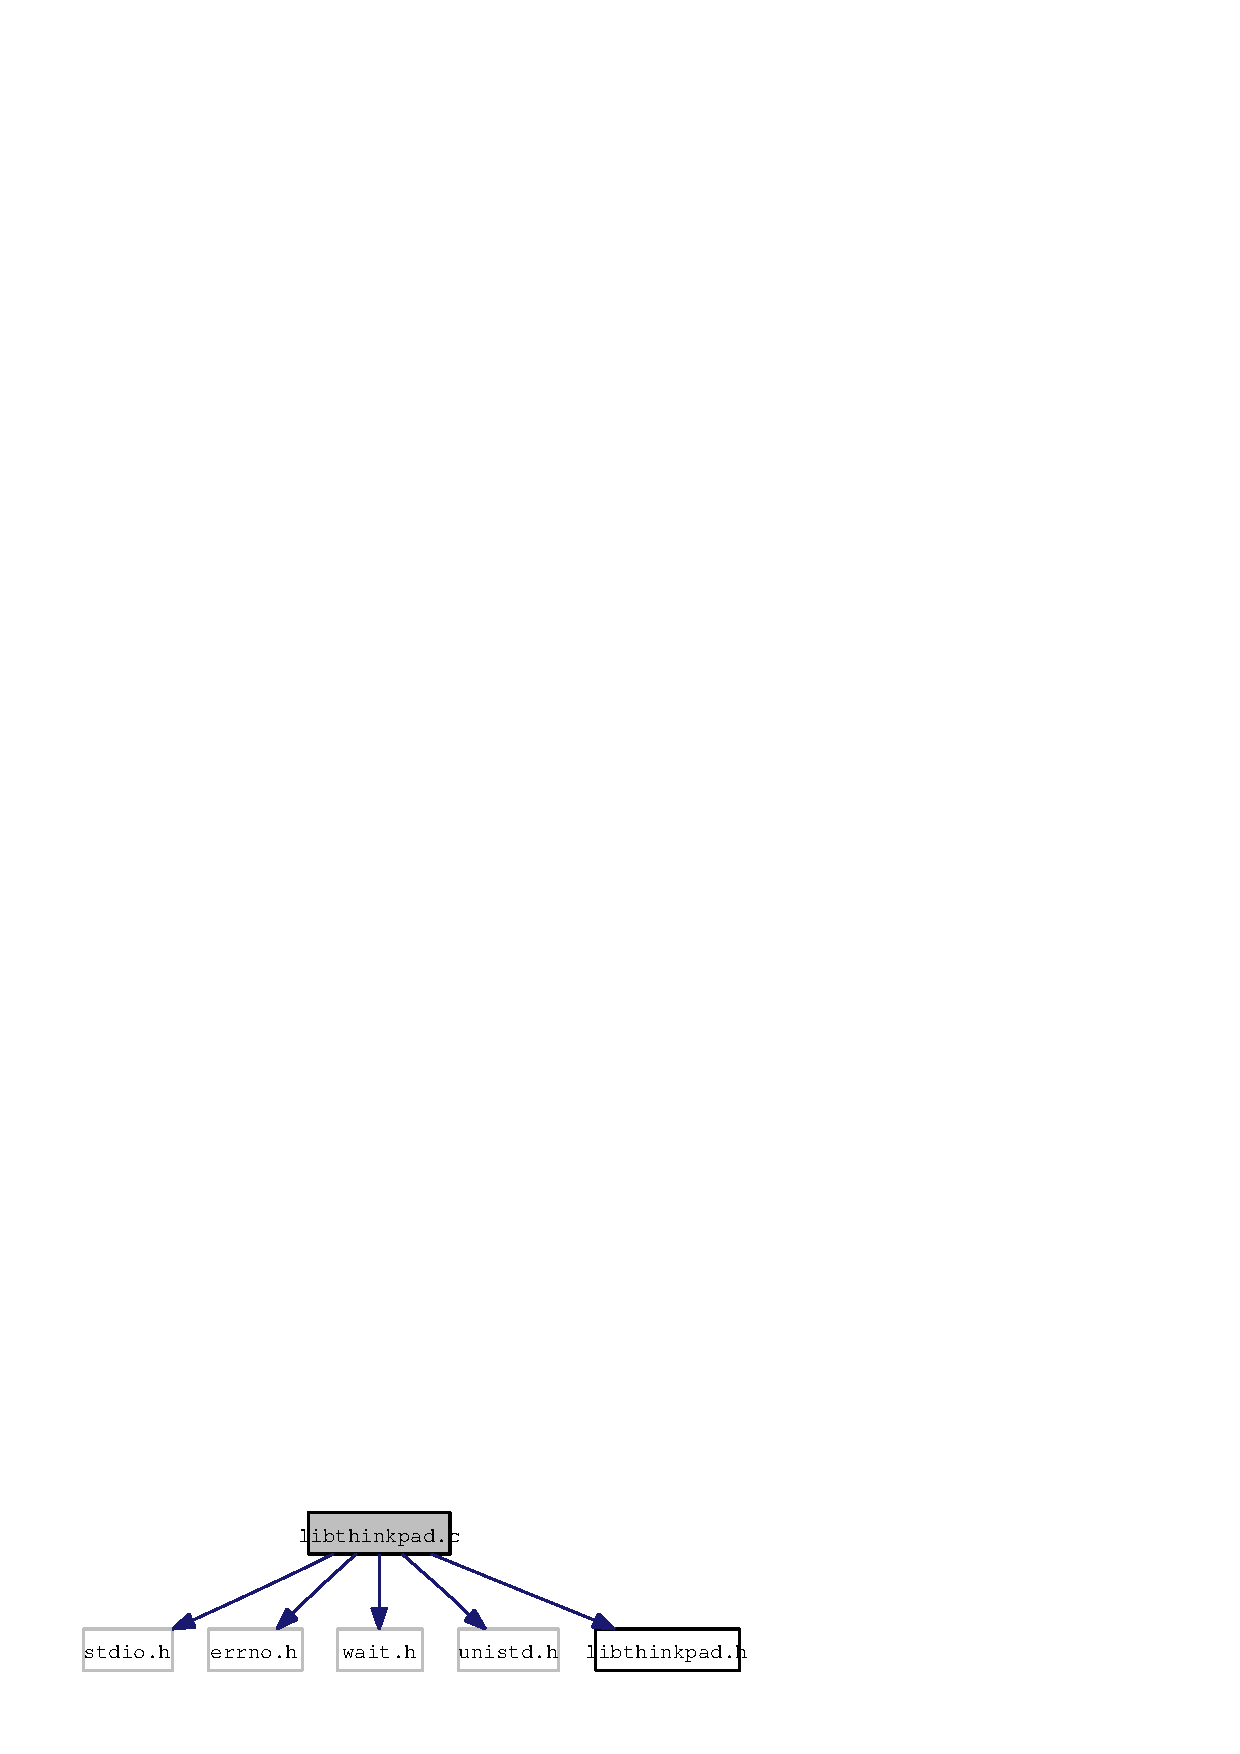
\includegraphics[width=179pt]{libthinkpad_8c__incl}
\end{center}
\end{figure}
\subsection*{Data Structures}
\begin{CompactItemize}
\item 
struct \hyperlink{structMorsecode}{Morsecode}
\end{CompactItemize}
\subsection*{Defines}
\begin{CompactItemize}
\item 
\#define \hyperlink{libthinkpad_8c_6eb92460cacc8cb18d42685f52181dd7}{MORSPOINT}~blinkLight(morse $\rightarrow$ point, 0, 1);
\item 
\#define \hyperlink{libthinkpad_8c_8c6f75e72798d81943388b4ef96fb7dd}{MORSLINE}~blinkLight(morse $\rightarrow$ line, 0, 1);
\end{CompactItemize}
\subsection*{Functions}
\begin{CompactItemize}
\item 
int \hyperlink{libthinkpad_8c_90f318656de4ddfd918141e20059474b}{blinkLight} (int on, int off, int num)
\item 
int \hyperlink{libthinkpad_8c_1c8a5a0db5fb813f149d4145c7d4a475}{blinkMorseChar} (char c)
\item 
int \hyperlink{libthinkpad_8c_b6b786c548e54b5dfc7697591c9211a6}{blinkMorseString} (char c\mbox{[}$\,$\mbox{]})
\end{CompactItemize}
\subsection*{Variables}
\begin{CompactItemize}
\item 
struct \hyperlink{structMorsecode}{Morsecode} \hyperlink{libthinkpad_8c_924cc52c5074766a5fa2ecce3c609d84}{morsecode}
\end{CompactItemize}


\subsection{Define Documentation}
\hypertarget{libthinkpad_8c_8c6f75e72798d81943388b4ef96fb7dd}{
\index{libthinkpad.c@{libthinkpad.c}!MORSLINE@{MORSLINE}}
\index{MORSLINE@{MORSLINE}!libthinkpad.c@{libthinkpad.c}}
\subsubsection{\setlength{\rightskip}{0pt plus 5cm}\#define MORSLINE~blinkLight(morse $\rightarrow$ line, 0, 1);}}
\label{libthinkpad_8c_8c6f75e72798d81943388b4ef96fb7dd}




Definition at line 37 of file libthinkpad.c.

Referenced by blinkMorseChar().\hypertarget{libthinkpad_8c_6eb92460cacc8cb18d42685f52181dd7}{
\index{libthinkpad.c@{libthinkpad.c}!MORSPOINT@{MORSPOINT}}
\index{MORSPOINT@{MORSPOINT}!libthinkpad.c@{libthinkpad.c}}
\subsubsection{\setlength{\rightskip}{0pt plus 5cm}\#define MORSPOINT~blinkLight(morse $\rightarrow$ point, 0, 1);}}
\label{libthinkpad_8c_6eb92460cacc8cb18d42685f52181dd7}




Definition at line 36 of file libthinkpad.c.

Referenced by blinkMorseChar().

\subsection{Function Documentation}
\hypertarget{libthinkpad_8c_90f318656de4ddfd918141e20059474b}{
\index{libthinkpad.c@{libthinkpad.c}!blinkLight@{blinkLight}}
\index{blinkLight@{blinkLight}!libthinkpad.c@{libthinkpad.c}}
\subsubsection{\setlength{\rightskip}{0pt plus 5cm}int blinkLight (int {\em on}, int {\em off}, int {\em num})}}
\label{libthinkpad_8c_90f318656de4ddfd918141e20059474b}


Switch the light over the lcd on and off (blinking).

\begin{Desc}
\item[Parameters:]
\begin{description}
\item[{\em on}]The time how long the light is switched on \item[{\em off}]The time how long the light is switched off \item[{\em num}]How often the light switching between on and off\end{description}
\end{Desc}
\begin{Desc}
\item[Returns:]The return value is 0 if all is okay or -1 if they was an error \end{Desc}


Definition at line 50 of file libthinkpad.c.

References LIGHTPROC.

Referenced by main().

Here is the caller graph for this function:\nopagebreak
\begin{figure}[H]
\begin{center}
\leavevmode
\includegraphics[width=87pt]{libthinkpad_8c_90f318656de4ddfd918141e20059474b_icgraph}
\end{center}
\end{figure}
\hypertarget{libthinkpad_8c_1c8a5a0db5fb813f149d4145c7d4a475}{
\index{libthinkpad.c@{libthinkpad.c}!blinkMorseChar@{blinkMorseChar}}
\index{blinkMorseChar@{blinkMorseChar}!libthinkpad.c@{libthinkpad.c}}
\subsubsection{\setlength{\rightskip}{0pt plus 5cm}int blinkMorseChar (char {\em c})}}
\label{libthinkpad_8c_1c8a5a0db5fb813f149d4145c7d4a475}


This function takes a char, and blinks than the letter in morsecode. \hyperlink{structMorsecode}{Morsecode} (\char`\"{}.\char`\"{} = short alias point, \char`\"{}-\char`\"{} = long alias line):

a -$>$ .- n -$>$ -. b -$>$ -... o -$>$ --- c -$>$ -.-. p -$>$ .--. d -$>$ -.. q -$>$ --.- e -$>$ . r -$>$ .-. f -$>$ ..-. s -$>$ ... g -$>$ --. t -$>$ - h -$>$ .... u -$>$ ..- i -$>$ .. v -$>$ ...- j -$>$ .--- w -$>$ .-- k -$>$ -.- x -$>$ -..- l -$>$ .-.. y -$>$ -.-- m -$>$ -- z -$>$ --..

1 -$>$ .---- 6 -$>$ -.... 2 -$>$ ..--- 7 -$>$ --... 3 -$>$ ...-- 8 -$>$ ---.. 4 -$>$ ....- 9 -$>$ ----. 5 -$>$ ..... 0 -$>$ -----

\begin{Desc}
\item[Parameters:]
\begin{description}
\item[{\em c}]The char for the morsecode\end{description}
\end{Desc}
\begin{Desc}
\item[Returns:]int The return value is 0 if all is okay or -1 if they was an error \end{Desc}


Definition at line 75 of file libthinkpad.c.

References Morsecode::line, morsecode, MORSLINE, MORSPOINT, Morsecode::pause, Morsecode::pausechar, Morsecode::pauseword, and Morsecode::point.

Referenced by blinkMorseString(), and main().

Here is the caller graph for this function:\nopagebreak
\begin{figure}[H]
\begin{center}
\leavevmode
\includegraphics[width=161pt]{libthinkpad_8c_1c8a5a0db5fb813f149d4145c7d4a475_icgraph}
\end{center}
\end{figure}
\hypertarget{libthinkpad_8c_b6b786c548e54b5dfc7697591c9211a6}{
\index{libthinkpad.c@{libthinkpad.c}!blinkMorseString@{blinkMorseString}}
\index{blinkMorseString@{blinkMorseString}!libthinkpad.c@{libthinkpad.c}}
\subsubsection{\setlength{\rightskip}{0pt plus 5cm}int blinkMorseString (char {\em c}\mbox{[}$\,$\mbox{]})}}
\label{libthinkpad_8c_b6b786c548e54b5dfc7697591c9211a6}




Definition at line 407 of file libthinkpad.c.

References blinkMorseChar(), Morsecode::line, morsecode, Morsecode::pause, Morsecode::pausechar, Morsecode::pauseword, and Morsecode::point.

Referenced by main().

Here is the call graph for this function:\nopagebreak
\begin{figure}[H]
\begin{center}
\leavevmode
\includegraphics[width=125pt]{libthinkpad_8c_b6b786c548e54b5dfc7697591c9211a6_cgraph}
\end{center}
\end{figure}


Here is the caller graph for this function:\nopagebreak
\begin{figure}[H]
\begin{center}
\leavevmode
\includegraphics[width=102pt]{libthinkpad_8c_b6b786c548e54b5dfc7697591c9211a6_icgraph}
\end{center}
\end{figure}


\subsection{Variable Documentation}
\hypertarget{libthinkpad_8c_924cc52c5074766a5fa2ecce3c609d84}{
\index{libthinkpad.c@{libthinkpad.c}!morsecode@{morsecode}}
\index{morsecode@{morsecode}!libthinkpad.c@{libthinkpad.c}}
\subsubsection{\setlength{\rightskip}{0pt plus 5cm}struct {\bf Morsecode}  {\bf morsecode}}}
\label{libthinkpad_8c_924cc52c5074766a5fa2ecce3c609d84}




Referenced by blinkMorseChar(), and blinkMorseString().
\hypertarget{libthinkpad_8h}{
\section{libthinkpad.h File Reference}
\label{libthinkpad_8h}\index{libthinkpad.h@{libthinkpad.h}}
}




This graph shows which files directly or indirectly include this file:\nopagebreak
\begin{figure}[H]
\begin{center}
\leavevmode
\includegraphics[width=102pt]{libthinkpad_8h__dep__incl}
\end{center}
\end{figure}
\subsection*{Defines}
\begin{CompactItemize}
\item 
\#define \hyperlink{libthinkpad_8h_4c0cbefe7ca00462bb109b7968fe272d}{LIGHTPROC}~\char`\"{}/proc/acpi/ibm/light\char`\"{}
\end{CompactItemize}
\subsection*{Functions}
\begin{CompactItemize}
\item 
int \hyperlink{libthinkpad_8h_90f318656de4ddfd918141e20059474b}{blinkLight} (int on, int off, int num)
\item 
int \hyperlink{libthinkpad_8h_1c8a5a0db5fb813f149d4145c7d4a475}{blinkMorseChar} (char c)
\item 
int \hyperlink{libthinkpad_8h_f42de626f64ff9ca399eb971d8cd07c1}{blinkMorseString} (char $\ast$c)
\end{CompactItemize}


\subsection{Define Documentation}
\hypertarget{libthinkpad_8h_4c0cbefe7ca00462bb109b7968fe272d}{
\index{libthinkpad.h@{libthinkpad.h}!LIGHTPROC@{LIGHTPROC}}
\index{LIGHTPROC@{LIGHTPROC}!libthinkpad.h@{libthinkpad.h}}
\subsubsection{\setlength{\rightskip}{0pt plus 5cm}\#define LIGHTPROC~\char`\"{}/proc/acpi/ibm/light\char`\"{}}}
\label{libthinkpad_8h_4c0cbefe7ca00462bb109b7968fe272d}




Definition at line 22 of file libthinkpad.h.

Referenced by blinkLight(), and help\_\-function().

\subsection{Function Documentation}
\hypertarget{libthinkpad_8h_90f318656de4ddfd918141e20059474b}{
\index{libthinkpad.h@{libthinkpad.h}!blinkLight@{blinkLight}}
\index{blinkLight@{blinkLight}!libthinkpad.h@{libthinkpad.h}}
\subsubsection{\setlength{\rightskip}{0pt plus 5cm}int blinkLight (int {\em on}, int {\em off}, int {\em num})}}
\label{libthinkpad_8h_90f318656de4ddfd918141e20059474b}


Switch the light over the lcd on and off (blinking).

\begin{Desc}
\item[Parameters:]
\begin{description}
\item[{\em on}]The time how long the light is switched on \item[{\em off}]The time how long the light is switched off \item[{\em num}]How often the light switching between on and off\end{description}
\end{Desc}
\begin{Desc}
\item[Returns:]The return value is 0 if all is okay or -1 if they was an error \end{Desc}


Definition at line 50 of file libthinkpad.c.

References LIGHTPROC.

Referenced by main().

Here is the caller graph for this function:\nopagebreak
\begin{figure}[H]
\begin{center}
\leavevmode
\includegraphics[width=87pt]{libthinkpad_8h_90f318656de4ddfd918141e20059474b_icgraph}
\end{center}
\end{figure}
\hypertarget{libthinkpad_8h_1c8a5a0db5fb813f149d4145c7d4a475}{
\index{libthinkpad.h@{libthinkpad.h}!blinkMorseChar@{blinkMorseChar}}
\index{blinkMorseChar@{blinkMorseChar}!libthinkpad.h@{libthinkpad.h}}
\subsubsection{\setlength{\rightskip}{0pt plus 5cm}int blinkMorseChar (char {\em c})}}
\label{libthinkpad_8h_1c8a5a0db5fb813f149d4145c7d4a475}


This function takes a char, and blinks than the letter in morsecode. \hyperlink{structMorsecode}{Morsecode} (\char`\"{}.\char`\"{} = short alias point, \char`\"{}-\char`\"{} = long alias line):

a -$>$ .- n -$>$ -. b -$>$ -... o -$>$ --- c -$>$ -.-. p -$>$ .--. d -$>$ -.. q -$>$ --.- e -$>$ . r -$>$ .-. f -$>$ ..-. s -$>$ ... g -$>$ --. t -$>$ - h -$>$ .... u -$>$ ..- i -$>$ .. v -$>$ ...- j -$>$ .--- w -$>$ .-- k -$>$ -.- x -$>$ -..- l -$>$ .-.. y -$>$ -.-- m -$>$ -- z -$>$ --..

1 -$>$ .---- 6 -$>$ -.... 2 -$>$ ..--- 7 -$>$ --... 3 -$>$ ...-- 8 -$>$ ---.. 4 -$>$ ....- 9 -$>$ ----. 5 -$>$ ..... 0 -$>$ -----

\begin{Desc}
\item[Parameters:]
\begin{description}
\item[{\em c}]The char for the morsecode\end{description}
\end{Desc}
\begin{Desc}
\item[Returns:]int The return value is 0 if all is okay or -1 if they was an error \end{Desc}


Definition at line 75 of file libthinkpad.c.

References Morsecode::line, morsecode, MORSLINE, MORSPOINT, Morsecode::pause, Morsecode::pausechar, Morsecode::pauseword, and Morsecode::point.

Referenced by blinkMorseString(), and main().

Here is the caller graph for this function:\nopagebreak
\begin{figure}[H]
\begin{center}
\leavevmode
\includegraphics[width=161pt]{libthinkpad_8h_1c8a5a0db5fb813f149d4145c7d4a475_icgraph}
\end{center}
\end{figure}
\hypertarget{libthinkpad_8h_f42de626f64ff9ca399eb971d8cd07c1}{
\index{libthinkpad.h@{libthinkpad.h}!blinkMorseString@{blinkMorseString}}
\index{blinkMorseString@{blinkMorseString}!libthinkpad.h@{libthinkpad.h}}
\subsubsection{\setlength{\rightskip}{0pt plus 5cm}int blinkMorseString (char $\ast$ {\em c})}}
\label{libthinkpad_8h_f42de626f64ff9ca399eb971d8cd07c1}



\hypertarget{thinkpadTest_8c}{
\section{thinkpadTest.c File Reference}
\label{thinkpadTest_8c}\index{thinkpadTest.c@{thinkpadTest.c}}
}


{\tt \#include $<$stdio.h$>$}\par
{\tt \#include $<$stdlib.h$>$}\par
{\tt \#include $<$string.h$>$}\par
{\tt \#include $<$errno.h$>$}\par
{\tt \#include $<$sys/types.h$>$}\par
{\tt \#include $<$unistd.h$>$}\par
{\tt \#include $<$signal.h$>$}\par
{\tt \#include $<$wait.h$>$}\par
{\tt \#include \char`\"{}libthinkpad.h\char`\"{}}\par


Include dependency graph for thinkpadTest.c:\nopagebreak
\begin{figure}[H]
\begin{center}
\leavevmode
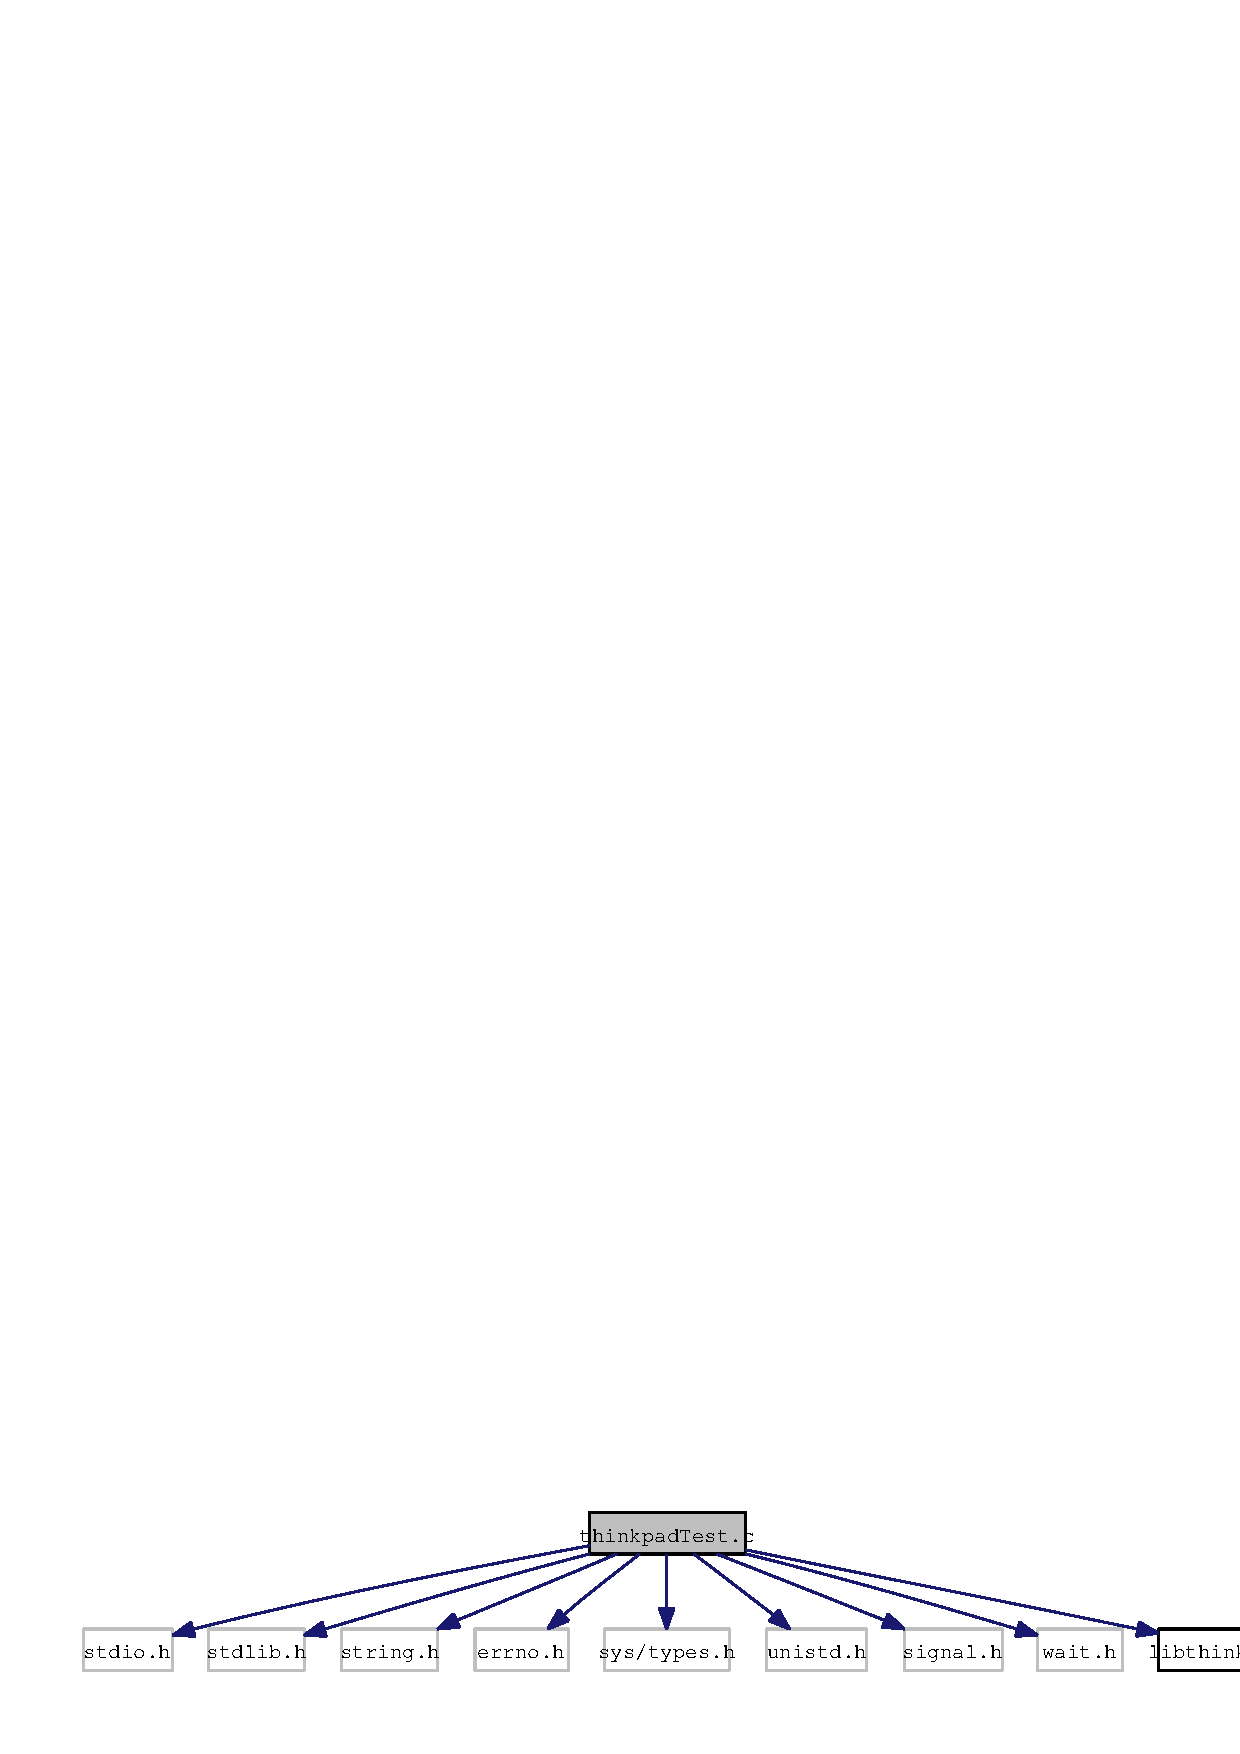
\includegraphics[width=314pt]{thinkpadTest_8c__incl}
\end{center}
\end{figure}
\subsection*{Defines}
\begin{CompactItemize}
\item 
\#define \hyperlink{thinkpadTest_8c_735563036dced0b7d6cc98f97ea4978b}{ERR}~error\_\-handler
\item 
\#define \hyperlink{thinkpadTest_8c_d61c6e0b19ce1ad5cd8846abc3fb21b7}{STRLENGTH}~1024
\item 
\#define \hyperlink{thinkpadTest_8c_a93f0eb578d23995850d61f7d61c55c1}{FALSE}~0
\item 
\#define \hyperlink{thinkpadTest_8c_a8cecfc5c5c054d2875c03e77b7be15d}{TRUE}~!FALSE
\end{CompactItemize}
\subsection*{Typedefs}
\begin{CompactItemize}
\item 
typedef int \hyperlink{thinkpadTest_8c_621c38f1f10a1c565d897e3178b16d6e}{boolean}
\end{CompactItemize}
\subsection*{Functions}
\begin{CompactItemize}
\item 
int \hyperlink{thinkpadTest_8c_da2823036b025c54a023335c757a6ae7}{error\_\-handler} (char $\ast$fctname, int errornb)
\item 
int \hyperlink{thinkpadTest_8c_2a3542d20c2ebfa5fbc7e21e49d6fa77}{help\_\-function} (int argc, char $\ast$argv\mbox{[}$\,$\mbox{]})
\item 
void \hyperlink{thinkpadTest_8c_38c50645b14fe30ab63098bc596f8a5b}{showWarranty} ()
\item 
void \hyperlink{thinkpadTest_8c_1cee2421b716d16a38e833923a3e2698}{showLicense} ()
\item 
int \hyperlink{thinkpadTest_8c_0ddf1224851353fc92bfbff6f499fa97}{main} (int argc, char $\ast$argv\mbox{[}$\,$\mbox{]})
\end{CompactItemize}


\subsection{Define Documentation}
\hypertarget{thinkpadTest_8c_735563036dced0b7d6cc98f97ea4978b}{
\index{thinkpadTest.c@{thinkpadTest.c}!ERR@{ERR}}
\index{ERR@{ERR}!thinkpadTest.c@{thinkpadTest.c}}
\subsubsection{\setlength{\rightskip}{0pt plus 5cm}\#define ERR~error\_\-handler}}
\label{thinkpadTest_8c_735563036dced0b7d6cc98f97ea4978b}




Definition at line 32 of file thinkpadTest.c.\hypertarget{thinkpadTest_8c_a93f0eb578d23995850d61f7d61c55c1}{
\index{thinkpadTest.c@{thinkpadTest.c}!FALSE@{FALSE}}
\index{FALSE@{FALSE}!thinkpadTest.c@{thinkpadTest.c}}
\subsubsection{\setlength{\rightskip}{0pt plus 5cm}\#define FALSE~0}}
\label{thinkpadTest_8c_a93f0eb578d23995850d61f7d61c55c1}




Definition at line 36 of file thinkpadTest.c.\hypertarget{thinkpadTest_8c_d61c6e0b19ce1ad5cd8846abc3fb21b7}{
\index{thinkpadTest.c@{thinkpadTest.c}!STRLENGTH@{STRLENGTH}}
\index{STRLENGTH@{STRLENGTH}!thinkpadTest.c@{thinkpadTest.c}}
\subsubsection{\setlength{\rightskip}{0pt plus 5cm}\#define STRLENGTH~1024}}
\label{thinkpadTest_8c_d61c6e0b19ce1ad5cd8846abc3fb21b7}




Definition at line 34 of file thinkpadTest.c.\hypertarget{thinkpadTest_8c_a8cecfc5c5c054d2875c03e77b7be15d}{
\index{thinkpadTest.c@{thinkpadTest.c}!TRUE@{TRUE}}
\index{TRUE@{TRUE}!thinkpadTest.c@{thinkpadTest.c}}
\subsubsection{\setlength{\rightskip}{0pt plus 5cm}\#define TRUE~!FALSE}}
\label{thinkpadTest_8c_a8cecfc5c5c054d2875c03e77b7be15d}




Definition at line 37 of file thinkpadTest.c.

\subsection{Typedef Documentation}
\hypertarget{thinkpadTest_8c_621c38f1f10a1c565d897e3178b16d6e}{
\index{thinkpadTest.c@{thinkpadTest.c}!boolean@{boolean}}
\index{boolean@{boolean}!thinkpadTest.c@{thinkpadTest.c}}
\subsubsection{\setlength{\rightskip}{0pt plus 5cm}typedef int {\bf boolean}}}
\label{thinkpadTest_8c_621c38f1f10a1c565d897e3178b16d6e}




Definition at line 39 of file thinkpadTest.c.

\subsection{Function Documentation}
\hypertarget{thinkpadTest_8c_da2823036b025c54a023335c757a6ae7}{
\index{thinkpadTest.c@{thinkpadTest.c}!error\_\-handler@{error\_\-handler}}
\index{error\_\-handler@{error\_\-handler}!thinkpadTest.c@{thinkpadTest.c}}
\subsubsection{\setlength{\rightskip}{0pt plus 5cm}int error\_\-handler (char $\ast$ {\em fctname}, int {\em errornb})}}
\label{thinkpadTest_8c_da2823036b025c54a023335c757a6ae7}




Definition at line 108 of file thinkpadTest.c.\hypertarget{thinkpadTest_8c_2a3542d20c2ebfa5fbc7e21e49d6fa77}{
\index{thinkpadTest.c@{thinkpadTest.c}!help\_\-function@{help\_\-function}}
\index{help\_\-function@{help\_\-function}!thinkpadTest.c@{thinkpadTest.c}}
\subsubsection{\setlength{\rightskip}{0pt plus 5cm}int help\_\-function (int {\em argc}, char $\ast$ {\em argv}\mbox{[}$\,$\mbox{]})}}
\label{thinkpadTest_8c_2a3542d20c2ebfa5fbc7e21e49d6fa77}




Definition at line 118 of file thinkpadTest.c.

References LIGHTPROC.

Referenced by main().

Here is the caller graph for this function:\nopagebreak
\begin{figure}[H]
\begin{center}
\leavevmode
\includegraphics[width=94pt]{thinkpadTest_8c_2a3542d20c2ebfa5fbc7e21e49d6fa77_icgraph}
\end{center}
\end{figure}
\hypertarget{thinkpadTest_8c_0ddf1224851353fc92bfbff6f499fa97}{
\index{thinkpadTest.c@{thinkpadTest.c}!main@{main}}
\index{main@{main}!thinkpadTest.c@{thinkpadTest.c}}
\subsubsection{\setlength{\rightskip}{0pt plus 5cm}int main (int {\em argc}, char $\ast$ {\em argv}\mbox{[}$\,$\mbox{]})}}
\label{thinkpadTest_8c_0ddf1224851353fc92bfbff6f499fa97}




Definition at line 49 of file thinkpadTest.c.

References blinkLight(), blinkMorseChar(), blinkMorseString(), help\_\-function(), showLicense(), and showWarranty().

Here is the call graph for this function:\nopagebreak
\begin{figure}[H]
\begin{center}
\leavevmode
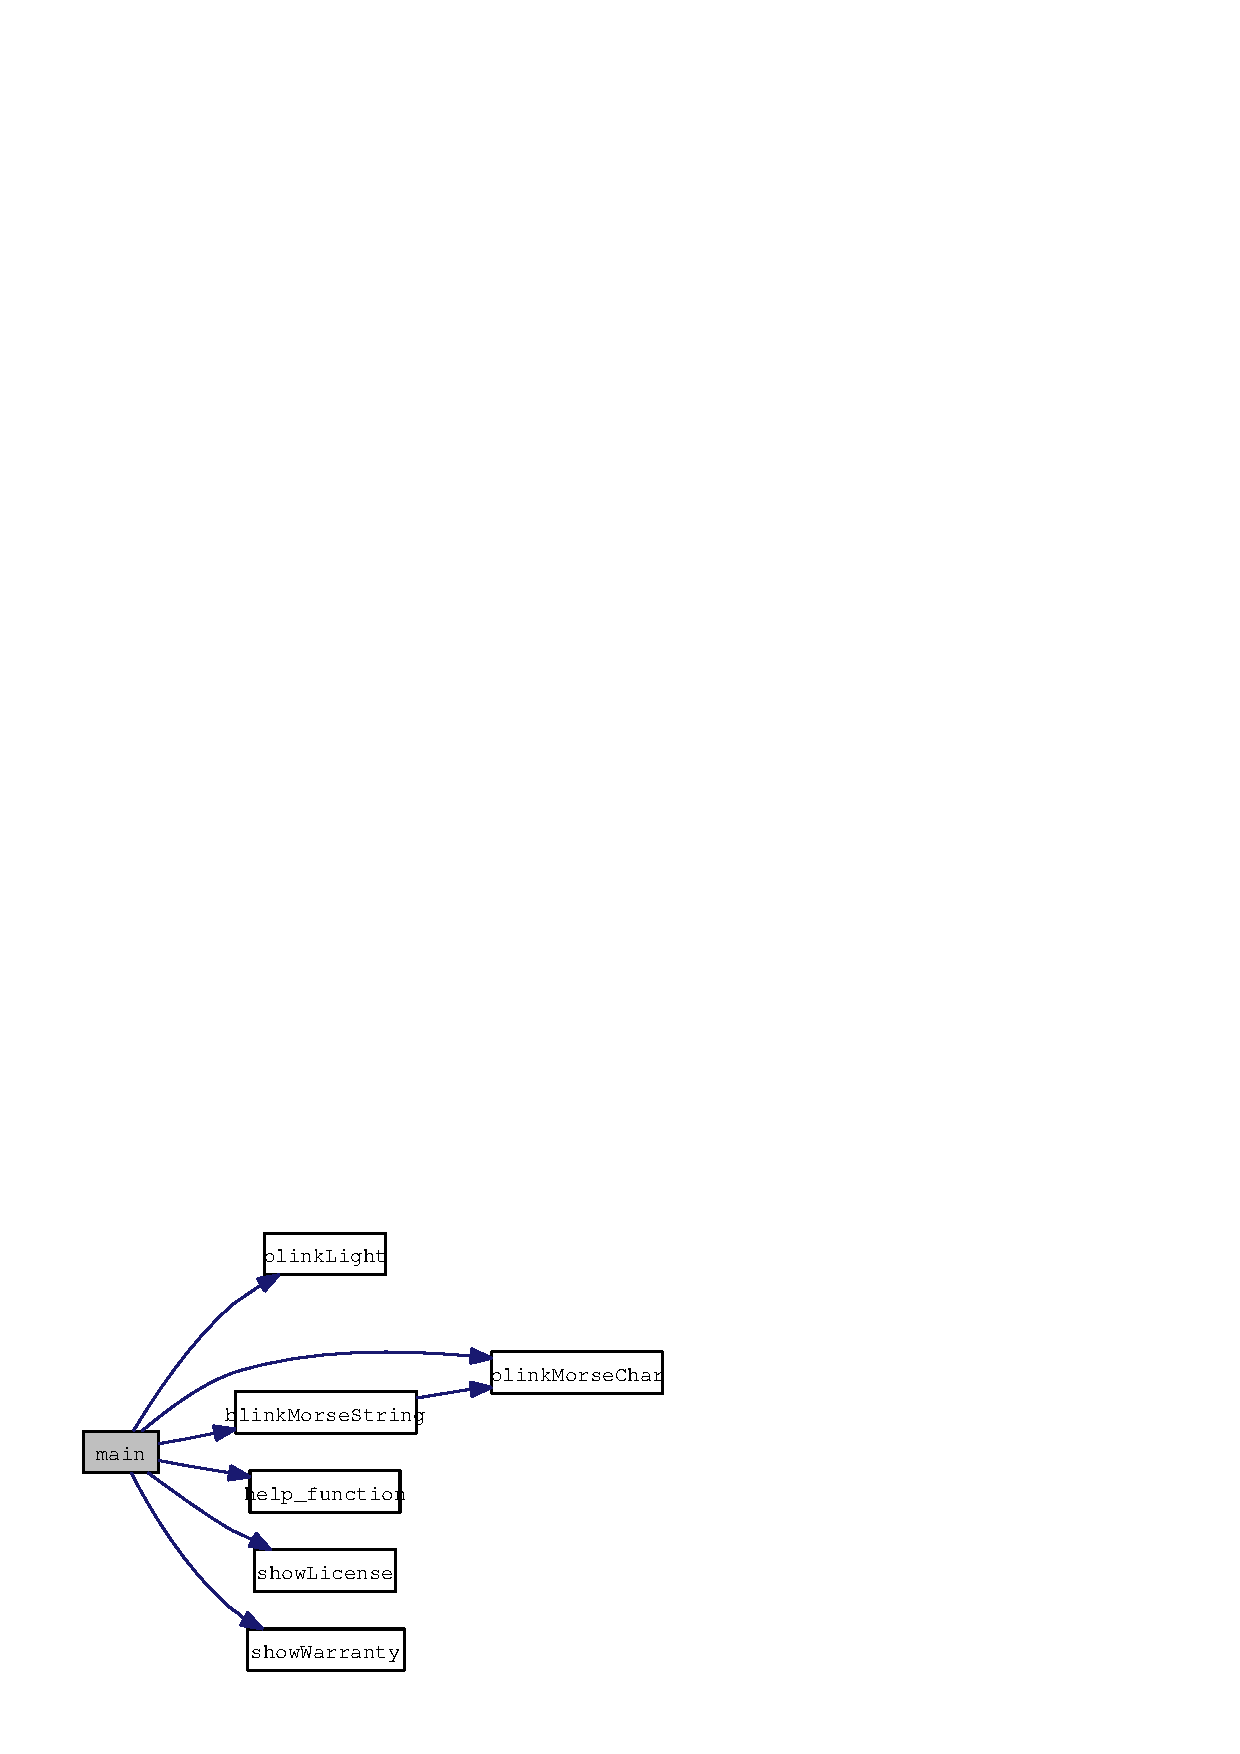
\includegraphics[width=161pt]{thinkpadTest_8c_0ddf1224851353fc92bfbff6f499fa97_cgraph}
\end{center}
\end{figure}
\hypertarget{thinkpadTest_8c_1cee2421b716d16a38e833923a3e2698}{
\index{thinkpadTest.c@{thinkpadTest.c}!showLicense@{showLicense}}
\index{showLicense@{showLicense}!thinkpadTest.c@{thinkpadTest.c}}
\subsubsection{\setlength{\rightskip}{0pt plus 5cm}void showLicense ()}}
\label{thinkpadTest_8c_1cee2421b716d16a38e833923a3e2698}




Definition at line 141 of file thinkpadTest.c.

Referenced by main().

Here is the caller graph for this function:\nopagebreak
\begin{figure}[H]
\begin{center}
\leavevmode
\includegraphics[width=92pt]{thinkpadTest_8c_1cee2421b716d16a38e833923a3e2698_icgraph}
\end{center}
\end{figure}
\hypertarget{thinkpadTest_8c_38c50645b14fe30ab63098bc596f8a5b}{
\index{thinkpadTest.c@{thinkpadTest.c}!showWarranty@{showWarranty}}
\index{showWarranty@{showWarranty}!thinkpadTest.c@{thinkpadTest.c}}
\subsubsection{\setlength{\rightskip}{0pt plus 5cm}void showWarranty ()}}
\label{thinkpadTest_8c_38c50645b14fe30ab63098bc596f8a5b}




Definition at line 137 of file thinkpadTest.c.

Referenced by main().

Here is the caller graph for this function:\nopagebreak
\begin{figure}[H]
\begin{center}
\leavevmode
\includegraphics[width=96pt]{thinkpadTest_8c_38c50645b14fe30ab63098bc596f8a5b_icgraph}
\end{center}
\end{figure}

\printindex
\end{document}
